\documentclass{beamer}
\mode<presentation>
\usetheme{Malmoe}
%gets rid of bottom navigation bars
\setbeamertemplate{footline}[page number]{}

%gets rid of navigation symbols
\setbeamertemplate{navigation symbols}{}

\usepackage{comment}

\usepackage{listings}
\usepackage{color}
\definecolor{mauve}{rgb}{0.58,0,0.82}

\lstset{frame=tb,
  language=Python,
  showstringspaces=false,
  columns=flexible,
  basicstyle={\small\ttfamily},
  numbers=none,
  keywordstyle=\color{blue},
  stringstyle=\color{mauve},
  breaklines=true,
  breakatwhitespace=true,
  tabsize=4
}

\title{BrainBuilder}
\author{Luis Riquelme, Mike Gevaert}
\institute{Human Brain Project}
\date{\today}

\begin{document}

\begin{frame}
  \titlepage
\end{frame}

\section{Introduction}
\begin{frame}
  \frametitle{Scope}
  In Scope:
  \begin{itemize}
     \item Workflow breakdown into modules
     \item Modules are swappable
  \end{itemize}

  Out of Scope:
  \begin{itemize}
     \item Not showing boiler-plate
     \item Implementations are not scientifically accurate
     \item Not showing implementations
  \end{itemize}
\end{frame}

\section{Modules}

\begin{frame}
  \frametitle{Modularity in BlueBuilder}
  Each Module is
  \begin{itemize}
    \item Self-contained
    \begin{itemize}
       \item Need only to take required parameters
       \item Need only to output data in a specified format
    \end{itemize}
    \item Replaceable, individually or en-masse
    \item Usually created a 'Random' version, and a more complex to verify the inputs and outputs made sense
  \end{itemize}
\end{frame}

\begin{frame}
  \frametitle{Modules in BrainBuilder}

  From previous work, and help from Eilif and Jean-Denis, these are the current set of modules:
  \begin{itemize}
     \item Build.Region: Select/Create Region of Interest (ROI)
     \item Build.Cells:  Cell Positions
     \item Build.EI:  E-I ratios
     \item Build.Composition.ME: METype for Soma
     \item Build.Placement: Morphology assignment
     \item Build.S2F: Functional Synapses (TBD)
     \item Build.NF: Channel Distribution (TBD)
     \item Build.SF: Synapse Functionality (TBD)
  \end{itemize}
\end{frame}

\subsection{Build.Region}
\begin{frame}[fragile]
  \frametitle{Build.Region: Region of Interest}

  Select region of interest by brain region or geometric primitives

  Example:
\begin{lstlisting}
from brainbuilder.select_region import select_region

region_name = 'Primary somatosensory area, lower limb'
roi = select_region(aibs_annotation, aibs_full_density, aibs_hierarchy, region_name)
\end{lstlisting}

  Outputs:
  \framebox{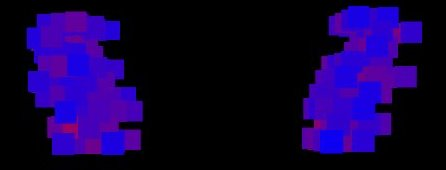
\includegraphics[width=\textheight]{images/region_selection.jpg}}
\end{frame}

\subsection{Build.Cells}
\begin{frame}[fragile]
  \frametitle{Build.Cells: Cell Positions}
  Generate a list of points within the ROI

  Example:
\begin{lstlisting}
from brainbuilder.cell_positioning import cell_positioning
positions = cell_positioning(roi, voxel_dimensions, total_cell_count)
\end{lstlisting}

  Outputs:
  \framebox{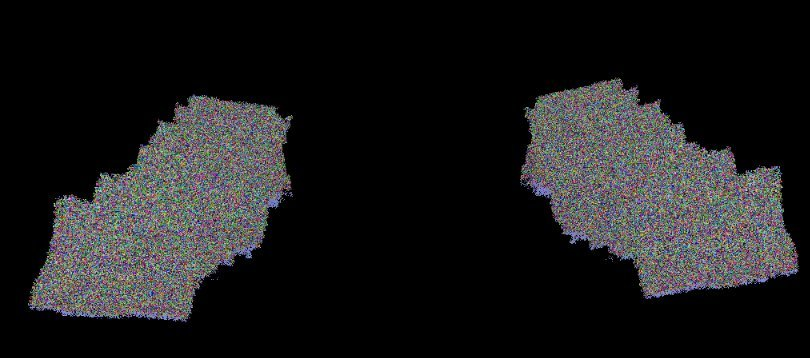
\includegraphics[width=\textheight]{images/cell_positions.jpg}}
\end{frame}

\subsection{Build.EI}
\begin{frame}[fragile]
  \frametitle{Build.EI: E-I Assignment - Random Assignment from Ratio}
  Assign each cell position it's E-I-ness
\begin{lstlisting}
from brainbuilder.assignment_synapse_class import assign_synapse_class_randomly
chosen_synapse_class = assign_synapse_class_randomly(positions, inhibitory_fraction=0.5)
\end{lstlisting}
  Outputs:
  \framebox{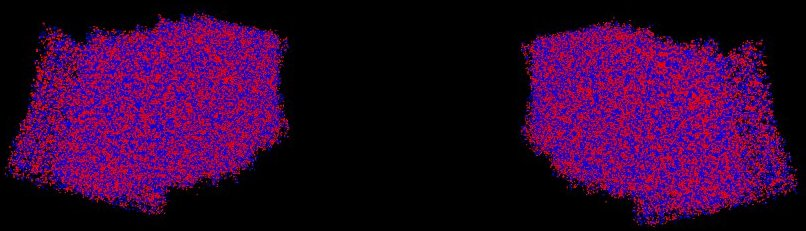
\includegraphics[width=\textheight]{images/sclass_random.jpg}}
\end{frame}

\begin{frame}[fragile]
  \frametitle{Build.EI: E-I Assignment - From Spatial Distribution}
  Example:
\begin{lstlisting}
from brainbuilder.assignment_synapse_class import assign_synapse_class_from_spatial_dist
chosen_synapse_class = assign_synapse_class_from_spatial_dist(positions, sclass_sdist, voxel_dimensions)
\end{lstlisting}
  Outputs:
  \framebox{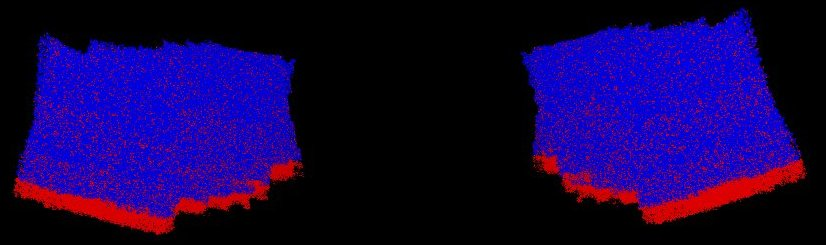
\includegraphics[width=\textheight]{images/sclass_spatial.jpg}}
\end{frame}

\subsection{Build.Composition.ME}
\begin{frame}[fragile]
  \frametitle{Build.Composition.ME: METype for Soma - Random}
  Assign each cell position ME-type
\begin{lstlisting}
from brainbuilder.assignment_metype import assign_metype_random
chosen_me = assign_metype_random(positions, mtypes, etypes)
\end{lstlisting}
  Outputs:
  \framebox{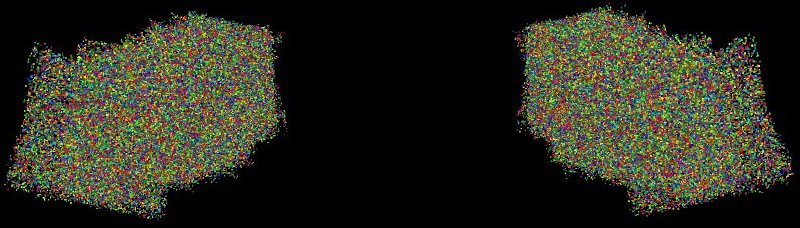
\includegraphics[width=\textheight]{images/mtype_random.jpg}}
\end{frame}

\begin{frame}[fragile]
  \frametitle{Build.Composition.ME: METype for Soma}
\begin{lstlisting}
from brainbuilder.assignment_metype import assign_metype
chosen_me = assign_metype(positions, chosen_synapse_class, recipe_sdist, voxel_dimensions)
\end{lstlisting}
  Outputs:
  \framebox{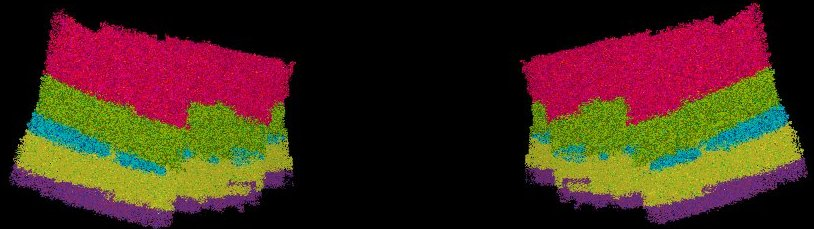
\includegraphics[width=\textheight]{images/mtype_recipe.jpg}}
\end{frame}

\subsection{Build.Placement}
\begin{comment}
\begin{frame}[fragile]
  \frametitle{Build.Placement: Morphology assignment - Random}
  Assignment each position a morphology 
\begin{lstlisting}
from brainbuilder.assignment_morphology import randomly_assign_morphology
chosen_morphology = randomly_assign_morphology(positions, morphologies)
\end{lstlisting}
  Outputs:
  \framebox{\includegraphics[width=\textheight]{images/random_metypes_positions.jpg}}
\end{frame}
\end{comment}

\begin{frame}[fragile]
  \frametitle{Build.Placement: Morphology assignment}
\begin{lstlisting}
from brainbuilder.assignment_morphology import assign_morphology
chosen_morphology = assign_morphology(positions, chosen_me, neuron_sdist, voxel_dimensions)
\end{lstlisting}
  Outputs:
  \framebox{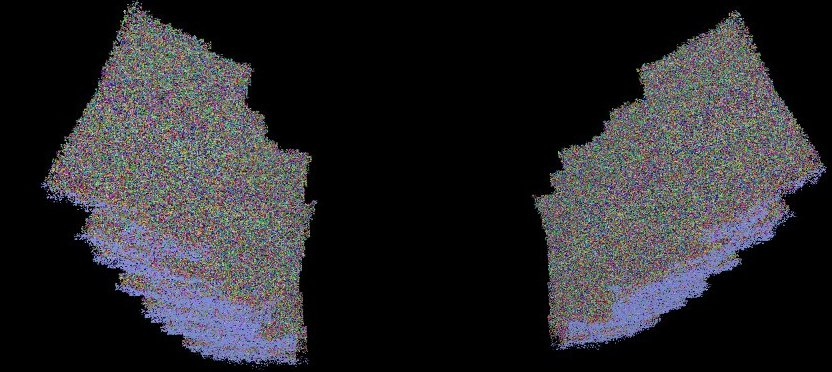
\includegraphics[width=\textheight]{images/morphs_recipe.jpg}}
\end{frame}

\section{Roadmap}
\begin{frame}
  \frametitle{Roadmap}

  \begin{itemize}
     \item Modules to be determined: need more scientific input
     \begin{itemize}
        \item Build.S2F: Functional Synapses
        \item Build.NF: Channel Distribution
        \item Build.SF: Synapse Functionality
        \item Note: MVD3
     \end{itemize}
     \item Standalone version
     \item GUI Controlled Version, integrated with the Collab
  \end{itemize}
\end{frame}

\end{document}
